Para o caso onde a artéria coronária possui aterosclerose,
o problema é modelado como um escoamento entre placas retas e paralelas
e curvadas. A geometria utilizada promove uma redução suave
da distância entre as paredes superior e inferior do canal.
Foi considerado 40\% de obstrução do canal devido a aterosclerose e
o domínio foi discretizado com 10261 nós e 23049 elementos triangulares lineares. \par
A \ref{velocity evolution curved} apresenta o perfil
de velocidade transiente ao longo da coordenada $y$ no
meio do canal ($x=5R$).
Como podemos observar, 
o valor adimensional máximo do campo de velocidade
chega a $u=2.3$ quando a artéria possui aterosclerose, isto é,
há um aumento de $53$\% da velocidade máxima quando comparado com
a artéria sem aterosclerose como apresentado na \ref{velocidade half poiseuille}.



\begin{figure}[H]
     \centering
     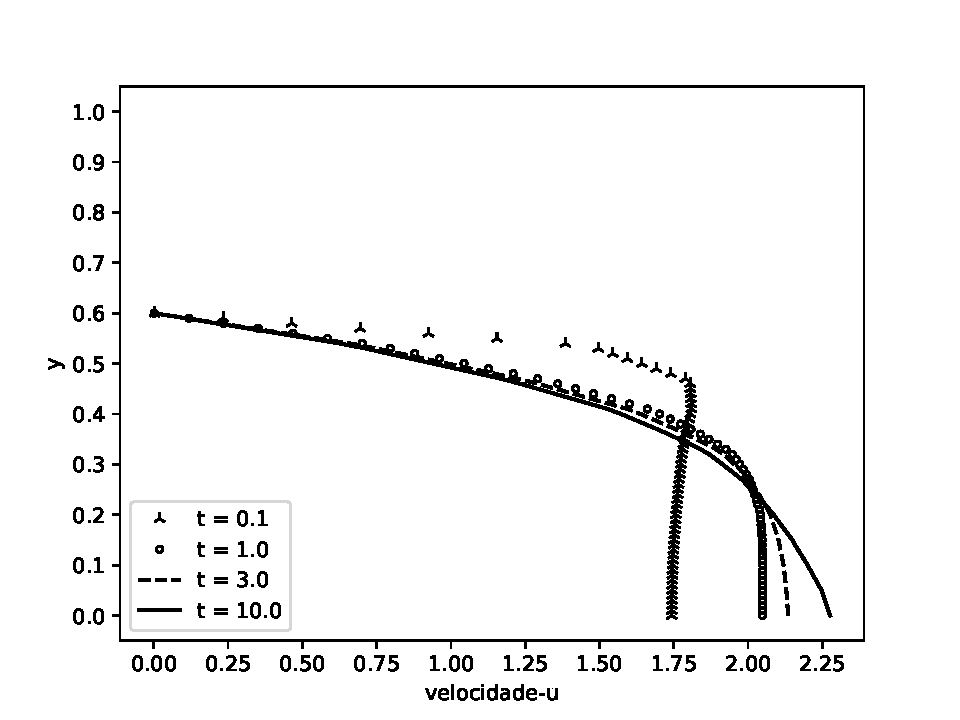
\includegraphics[scale=1]{./02_chaps/cap_solution/figure/vel_Curved_evol.pdf}\\
     \caption{Evolução no tempo do perfil da velocidade para o Canal Curvado.}
     \label{velocity evolution curved}
\end{figure}

\newpage
A \ref{velocity field curved} apresenta a evolução no tempo e no espaço
do campo de velocidade para a metade do domínio, pois os resultados são simétricos
na direção $y$. O campo de velocidade é representado com os valores adimensionais
onde a cor vermelha se refere ao valor $u=2.3$ e a cor azul $u=0$. Transformando em
valores dimensionais temos $u=27.6 cm/s$ e $u=0 cm/s$ respectivamente.

\vspace{2cm} 
\begin{figure}[H]
     \begin{minipage}{.50\linewidth}
      \centering
      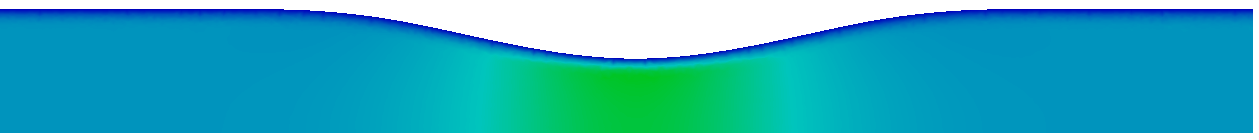
\includegraphics[scale=0.175]{./02_chaps/cap_solution/figure/vel_Curved200.png}\\
      t = 0.1
     \end{minipage}%
     \begin{minipage}{.50\linewidth}
      \centering
      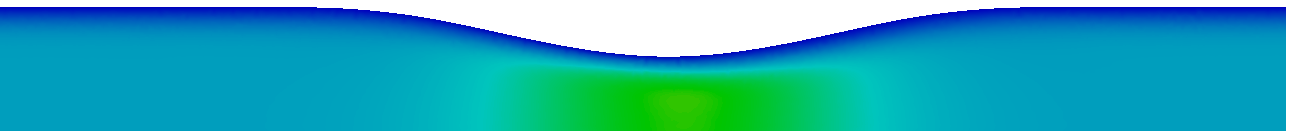
\includegraphics[scale=0.172]{./02_chaps/cap_solution/figure/vel_Curved1000.png}\\
      t = 0.5
     \end{minipage}
     \begin{minipage}{.50\linewidth}
     \medskip
      \centering
      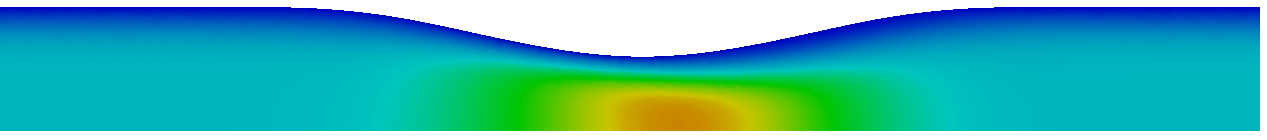
\includegraphics[scale=0.175]{./02_chaps/cap_solution/figure/vel_Curved2000.png}\\
      t = 1.0
     \end{minipage}%
     \begin{minipage}{.50\linewidth}
     \medskip
      \centering
      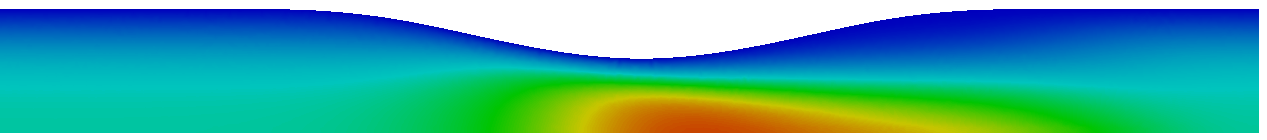
\includegraphics[scale=0.175]{./02_chaps/cap_solution/figure/vel_Curved6000.png}\\
      t = 3.0
     \end{minipage}
     \begin{minipage}{.50\linewidth}
      \centering
      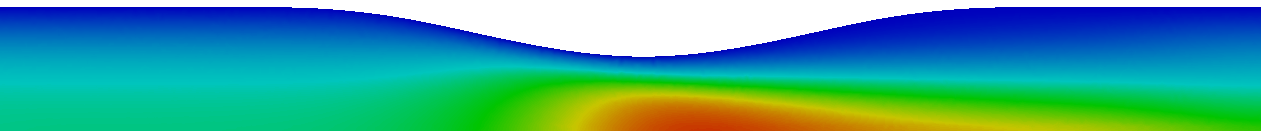
\includegraphics[scale=0.175]{./02_chaps/cap_solution/figure/vel_Curved8000.png}\\
      t = 4.0
     \end{minipage}%
     \begin{minipage}{.50\linewidth}
      \centering
      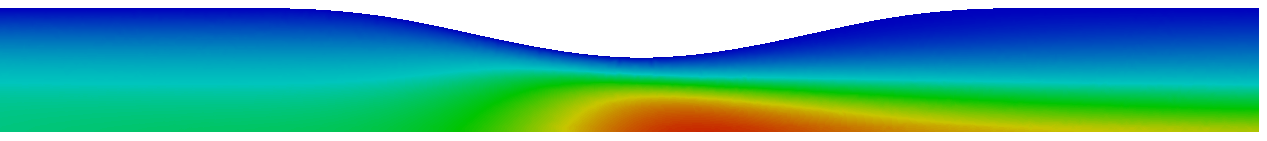
\includegraphics[scale=0.175]{./02_chaps/cap_solution/figure/vel_Curved10000.png}\\
      t = 5.0
     \end{minipage}
     \begin{minipage}{.50\linewidth}
     \medskip
      \centering
      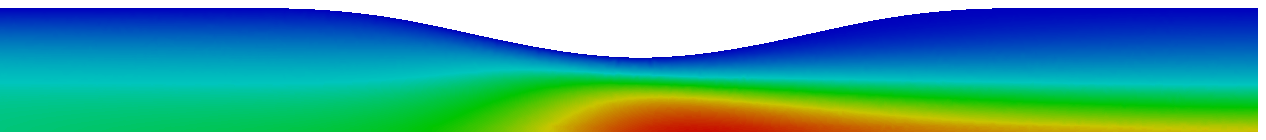
\includegraphics[scale=0.175]{./02_chaps/cap_solution/figure/vel_Curved14000.png}\\
      t = 7.0
     \end{minipage}%
     \begin{minipage}{.50\linewidth}
     \medskip
      \centering
      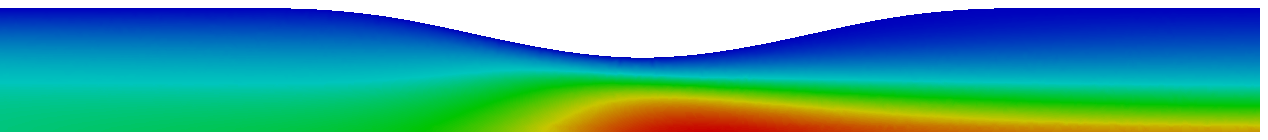
\includegraphics[scale=0.175]{./02_chaps/cap_solution/figure/vel_Curved20000.png}\\
      t = 10.0
     \end{minipage}
     \medskip
     \caption{Evolução no tempo e no espaço do campo de velocidade para o Canal Curvado.}
     \label{velocity field curved}
\end{figure}

\newpage
